\documentclass[modern]{aastex631}


\usepackage{amsmath}
\usepackage{amssymb}
\usepackage{hyperref}
\usepackage{bm}
\usepackage{listings}
\usepackage{graphicx}
\usepackage{float}
\usepackage{soul}
\usepackage{mathtools}
\usepackage{esint}

% missing figure command

\usepackage{blindtext}
\usepackage{graphicx}
\usepackage{tcolorbox}
\usepackage{fontawesome}
\usepackage{booktabs}

\definecolor{linkcolor}{rgb}{0.1216,0.4667,0.7059}


\let\StandardIncludeGraphics\includegraphics%
\renewcommand{\includegraphics}[2][]{%
\IfFileExists{#2}{%
  \StandardIncludeGraphics[#1]{#2}%
}{%
 \IfFileExists{#2.pdf}{%
  \StandardIncludeGraphics[#1]{#2}%
  }{ % No, no .pdf, try *.jpg 
   \IfFileExists{#2.jpg}{%
    \StandardIncludeGraphics[#1]{#2}%
    }{
      \IfFileExists{#2.png}{%
      \StandardIncludeGraphics[#1]{#2}%
      }{%
      \begin{tcolorbox}[width=6cm,height=4cm,arc=0mm,auto outer arc]
      \end{tcolorbox}
     }
   }
 }
}% 
%
}

% commands
\newcommand{\todo}[1]{\colorbox{red}{\textcolor{white}{\texttt{TO DO}}}\,}
\newcommand{\set}[1]{\{\,#1\,\}}
\newcommand{\footlink}[1]{\footnote{\url{#1}}}
\DeclareMathOperator*{\argmax}{arg\,max}
\DeclareMathOperator*{\argmin}{arg\,min}
\let\subsectionautorefname\sectionautorefname
\let\subsubsectionautorefname\sectionautorefname
\newcommand{\codeicon}{{\color{linkcolor}\faFileCodeO}}
\newcommand{\codelink}[1]{\href{https://github.com/lgrcia/paper-jaxoplanet/blob/main/#1.py}{\codeicon}\,\,}
\newcommand{\gitlink}{\href{https://github.com/lgrcia/paper-jaxoplanet}{\color{linkcolor}\faGithub}\,\,}

% no indent
\setlength\parindent{0pt}

% code style
\lstdefinestyle{mystyle}{
    backgroundcolor=\color{white},
    commentstyle=\color{gray!70},
    keywordstyle=\color{Bittersweet},
    stringstyle=\color{RoyalBlue},
    basicstyle=\fontsize{8.5}{13}\fontfamily{DejaVuSansMono-TLF}\selectfont,
    breakatwhitespace=false,         
    breaklines=true,
    rulecolor=\color{black!15},
    numbers=none,
    numberstyle=\fontsize{7}{11}\fontfamily{DejaVuSansMono-TLF}\selectfont\color{gray!50},
    framerule=0pt,
    breakindent=5pt,
    resetmargins=true,
    numbersep=10pt,
    frame=single,
    aboveskip=1em,
    belowskip=1em,
    xleftmargin=6pt,
    framexleftmargin=4pt
}
\lstset{style=mystyle}

\newcommand{\bvec}[1]{{\ensuremath{\mathbf{#1}}}}

\begin{document}

\title{\texttt{jaxoplanet}: Hardware-Accelerated Computation of Stellar Light Curves}

% author info
\author{Lionel J. Garcia}
\author{Soichiro Hattori}
\author{Daniel Foreman-Mackey}
\affiliation{Center for Computational Astrophysics, Flatiron Institute, New York, NY, USA}

\keywords{}

\begin{abstract}
    The measurement of stellar fluxes over time serves a wide variety of science cases. Transit and occultation light curves, for example, are used to characterize the orbital parameters of stellar systems, and infer the atmospheric properties of their transiting bodies. Phase curves, on the other hand, can be used to study the thermal emission of exoplanets, and the atmospheric circulation of stars. In order to infer these properties, a fast, accurate and robust model of stellar light curves is needed, one that accounts for the non-uniform surface intensity of spherical bodies and their mutual occultations. The analytical framework known as \textsf{starry} satisfies these requirements, and was successfully applied over the years following its development. However, as datasets and model complexity grow, the tractable inference of these parameters becomes increasingly challenging, and often motivates biased approximations. In this paper, we present a new implementation of the \textsf{starry} framework in \texttt{jax}, a high-performance machine-learning library designed for large-scale computations. We describe the changes made to the original version of \textsf{starry} and evaluate the performance of its new implementation that we release in the open-source Python package \textsf{jaxoplanet}. Through this implementation, we provide the community with a differentiable model of stellar light curves, and enable the use of powerful machine-learning tools available in the \texttt{jax} ecosystem. \gitlink{}

\end{abstract}

\section*{Introduction}


% the computation of \textit{starry} light curves can be computationally expensive, especially when considering the large number of parameters that need to be inferred from the data. In this paper, we present a new implementation of the \textit{starry} model that leverages the \texttt{jax} library to perform hardware-accelerated computations on GPUs. We show that this implementation can be used to compute light curves up to 100 times faster than the original implementation, and we demonstrate its application to the inference of the orbital parameters of exoplanets from transit light curves.



% Stellar light curves and radial velocity models provided an important tool to study exoplanetary systems. At the origin of these models lies the first principles of orbital mechanics, the Kepler equations, and the algorithms used to solve them. On top of that, models like Agol, of occultation light curves extended our capability to study these systems in greater details, using transits. In practice, computing this model and making inference based on these observables has been enabled by the implementation of these models with optimized frameworks and inference tools (pymc3), providing robust implementation of sampling algorithms and other inferrence tools. A good example of this synergy is the development of exoplanet and starry in c++ backed by Pymc3 which enabled major discoveries based on large datasets. With the recent lunch of JWST, we crumble under data. For example, transmission spectra on hundreds of channels, multi-planet systems and a large number of free parameters with their priors. At the same time, machine learning continue to grow, and novel framework appear and lead to application in physics. One of this framework is jax, developped by google, and gaining a huge popularity on the astronomy community. JAX is a hp machine-learning library that pre-compile code to LAX for paralilisation. It allows complex model to be written direclty in python, where usually a lower-level langage like C is preferable, and parallelised on CPU, GPU or any lax-compatible device. Not only it's good because of the higher level syntax of python that made it popular in science. But also because of the capability to run expansive models on GPU, a trend observed in other field of ML and DL where scaling is required.

% In this paper, we describe an implementation of the starry formalism in jax, allowing for the inference of a large number of parameters on complex models, exploiting the latest dev in ML machinery.

\newpage
\section{Light curve models}\label{starry}

Inspired by the idea of \cite{pal2012}, \cite{starry} and \cite{Agol2020} present a general framework to compute the light curves of spherical bodies with non-uniform surface intensities. This framework, known as \textit{starry}, allows for precise and efficient computation of the light curves of stars and exoplanets, and has been successfully applied to a wide variety of science cases. In this section, we describe the mathematical formalism behind the \textit{starry} model.

\subsection{Spherical harmonics}

The surface of a spherical body can be naturally described by spherical harmonics: a set of special functions defined on the sphere that can serve as orthonormal basis to represent any spherical surface map. If $\bvec{\tilde y}$ denotes the spherical harmonics basis of degree $l_{max}$ (defined in \citealt[section X]{starry}) and $\bvec{y}$ a vector that contains the coefficients describing the surface in this basis, the intensity $I$ of the map projected onto the sky-projected $(x, y)$ plane of the observer is
\begin{equation}I(x, y) = \bvec{\tilde y^\mathsf{T}}(x, y) \, \bvec{y}.\end{equation}
In order to orient this surface, for example with a given inclination, obliquity and phase around its rotation axis, we define a rotation matrix $\bvec{R}$ that acts on the spherical harmonics coefficients $\bvec{y}$, such that the intensity of the map projected onto the sky of the observer is
\begin{equation}I(x, y) = \bvec{\tilde y}^\mathsf{T}(x, y) \, \bvec{R} \, \bvec{y}.\end{equation}\\
\subsection{Rotation light curve}
Using this expression, the integrated intensity of the rotated map is
\begin{equation}F = \iint I(x,y)\,\text{d}S = \iint \bvec{\tilde y^\mathsf{T}}\bvec{R}\bvec{y}\,\text{d}S\end{equation}
In order to simplify this integral, \citealt{starry} introduce a change of basis from the spherical harmonics basis $\bvec{\tilde y}$ to a simple polynomial basis $\bvec{\tilde p}$ characterized by the change of basis matrix $\bvec{A_1}$. In this new basis, $\bvec{y}$ can be expressed as
\begin{equation}\bvec{p} = \bvec{A_1}\bvec{y},\end{equation}
such that 
\begin{equation}I(x, y) = \bvec{\tilde p^\mathsf{T}}(x, y)\,\bvec{A_1}\bvec{R}\bvec{y}.\end{equation}
Hence,
\begin{equation}F = \iint \bvec{\tilde p^\mathsf{T}}\bvec{A_1}\bvec{R}\bvec{y}\,\text{d}S = \bvec{r^\mathsf{T}}\bvec{A_1}\bvec{R}\bvec{y},\end{equation}
with
\begin{equation}\bvec{r^\mathsf{T}} \equiv \iint \mathbf{\tilde{p}}^\top\,\text{d}S,\end{equation}
since $\bvec{A_1}$, $\bvec{R}$ and $\bvec{y}$ are independent of the coordinates on the sphere.\\\\
As $\bvec{\tilde{p}}$ is simply made of polynomials of the coordinates $x$, $y$ and $z$, the elements of the \textit{rotation vector} $\bvec{r}$ can be computed analytically and only once for a given $l_{max}$ (see \citealt[Eq. 20]{starry}).\\\\
\subsection{Occultation light curve}
The same formalism can be used to compute the integrated intensity of a surface map occulted by another spherical body. In this case, the intensity of the map must be integrated only over the unocculted surface $S$ of the disk, such that 
\begin{equation} F = \iint_S I(x,y)\,\text{d}S = \left(\iint_S \bvec{\tilde p^\mathsf{T}}\,\text{d}S\right)\bvec{A_1}\bvec{R}\bvec{y}.\end{equation}
To simplify this expression, \citealt{pal2012} note that any two-dimensional integral of the unocculted disk can be reduced to a one-dimensional integral over the contour $C$ of the occulting body using Green's theorem\footnote{Also known as Stokes' theorem in three-dimensional vector calculus.}. This can be done if the integrand of the integral over S can be described by a function $f$ such that
\begin{equation}f(x, y) = \frac{\delta G_{y}}{\delta x}-\frac{\delta G_{x}}{\delta y},\end{equation}
where $G$ is a vector field defined and differentiable over $S$.\\\\
By applying a last change of basis matrix $\bvec{A_2}$ to the polynomial basis $\bvec{\tilde p}$, \citealt{starry} transforms $\bvec{\tilde p}$ to the \textit{Green's basis} $\bm{\tilde g}$ that satisfies this property, meaning that the surface integral of each of its components $\tilde{g_n}$ can be transformed to the line integral
\begin{equation}
    \label{eq:sn_gn}
    s_n \equiv \iint_S \tilde{g_n}(x, y)\,\text{d}S = \oint_C \bvec{G}_n(x, y)\,\text{d}\bvec{r},
\end{equation}
with $\bvec{G}_n$ given in \citealt[Equation 34]{starry}. These functions require the occulting body to be aligned with the $y$-axis of the reference frame, which can be achieved by applying a final rotation matrix $\bvec{R'}$ to the surface map.\\\\
Using these expressions, the integrated intensity of the occulted map follows the idiomatic linear expression 
\begin{equation}F = \bvec{s^\mathsf{T}}\bvec{A}\,\bvec{R'}\,\bvec{R}\,\bvec{y},\end{equation}
with $\bvec{A} = \bvec{A_2A_1}$ and the integrals $s_n$ arranged in the \textit{solution vector} $\bvec{s^\mathsf{T}}$.\\\\

\subsection{Limb-darkened surfaces}
We notice that a simpler situation is encountered when the surface of the spherical body can be described by a radial intensity profile $I(r)$, such as a limb-darkened star. In this case, the vector of spherical harmonics coefficients $\bvec{y}$ is very sparse (because all $m\neq0$ components are zero) and the surface map doesn't need to be rotated. Contemporary to \cite{starry}, \cite{Agol2020} explore this case and provide simple expressions for the integrated intensity of a star whose surface can be described by a polynomial limb-darkening law occulted by an opaque body. In this case:
\begin{enumerate}
    \item The surface is simply described by $\bvec{u}$, a vector of polynomial limb-darkening coefficients.
    \item The Green's basis takes a simpler form (see \citealt[Eq. X]{Agol2020}).
    \item Matrices involved in the computation of the integrated flux have $l_{max}$ columns, versus $(l_{max}+1)^2$ in the general case, reducing drastically the computational cost of the model.
\end{enumerate}
For these reasons, and because of its wide application, our implementation treats radially-symmetric maps separately, leading to highly optimize computations of limb-darkened light curves.\\\\


\newpage
\section{Implementation details}\label{optimization}
\subsection{Limb-darkening multiplicative maps}
\subsection{Spherical harmonics rotations}

% tldr: rotating SH involves costly matrices computations. Hence its smart to figure out which one to pre-compute. That what RL did, amd it led to 6 elementary rotations. However, now that we use jax we don't care that much, and we can reduce the all thing to a single rotation that is optimized at compiled time.\\\\

With \textit{starry}, every light curve computation at a given time $t$ involves a rotation of the spherical harmonics basis, from the rest-frame of the star (\autoref{fig:rotation_basis}, left) to its sky-projected orientation (\autoref{fig:rotation_basis}, right), with a final rotation relative to the position of the occulting body (see Figure 2. from \citealt{starry}).
\begin{figure}[H]
    \begin{center}
        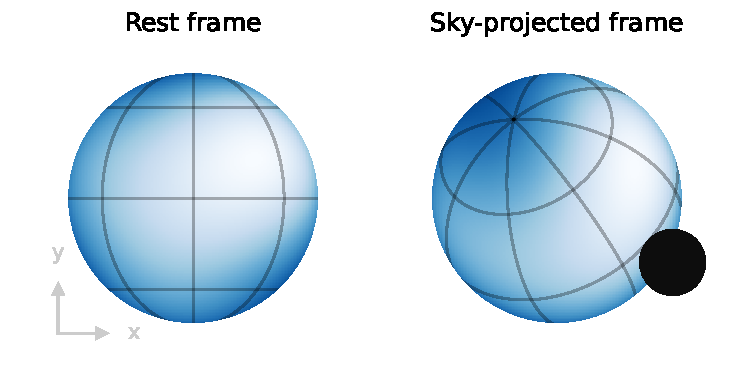
\includegraphics[width=0.6\textwidth]{../workflows/rotations/figures/rotation_basis.pdf}
        \caption{Rotation of the spherical harmonics basis to place the star in the sky-projected frame of the observer.}
        \label{fig:rotation_basis}
    \end{center}
\end{figure}

The rotation of spherical harmonics involves the computation of Wigner-D-matrices, commonly obtained through robust recursion relations in both degree $l$ and order $m$, but leading to costly computations. Hence, knowing how to decompose the full spherical harmonics rotation using pre-computed rotations is essential to achieve optimal performance in the \textit{starry} framework. \autoref{fig:rotation_starry} shows the 6 elementary rotations currently used in the \textsf{starry} implementation.
\begin{figure}[H]
    \begin{center}
        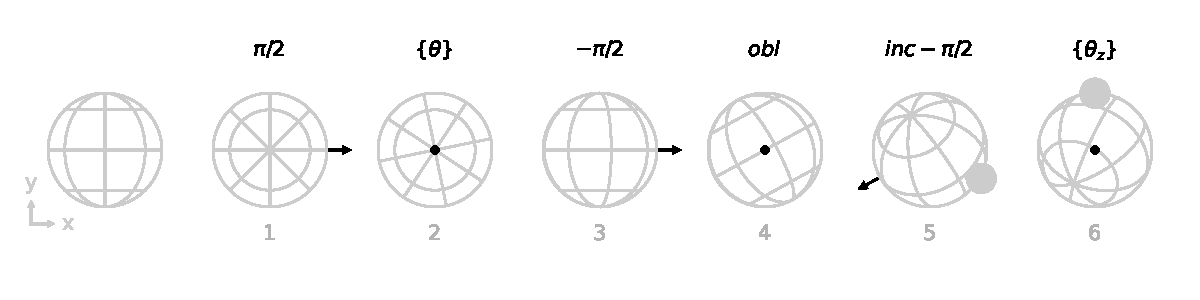
\includegraphics[width=\textwidth]{../workflows/rotations/figures/rotation_starry.pdf}
        \caption{Consecutive rotations of the spherical harmonics basis in the \textsf{starry} implementation. Each schematic shows a sphere rotated from a previous orientation around an axis displayed as a black vector and an angle shown on top.}
        \label{fig:rotation_starry}
    \end{center}
\end{figure}
In this figure, rotations 1 to 3 correspond to a rotation of the star around its rotation axis, and rotations 3 to 5 place the star on a sky-projected frame. Finally, rotation 6 aligns the spherical harmonics map to the occulting body on the $y$ axis in order to apply Green's theorem in the appropriate basis (Figure 2 from \citealt{starry}). The first thing to notice is that rotations 1 to 3 could be simply reduced to a rotation of angle $\theta$ about the y-axis, turning steps 1 to 3 into one. However, rotations around the pole, i.e.\,with a rotation axis along $z$, have simpler expressions that can be implemented separately. In addition, pre-computing these matrices at lower cost is particularly important for steps 2 and 6, involving a potentially large set of angles $\{\theta\}$ and $\{\theta_z\}$, defined over times $\{t\}$, for which to compute the full light curve. This explains the current decomposition of the complete rotation in six separate steps.\\\\
In \textsf{jaxoplanet}, we compute the Wigner-D-matrices by employing the Risbo recursion relations \citep{Risbo1996} implemented in \texttt{JAX} as part of the \texttt{s2fft} Python package \citep{price:s2fft}. In addition, we merge rotations 3, 4 and 5 (see \autoref{fig:rotation_jaxoplanet}) into a single compound rotation of axis
\begin{equation}
    \bvec{v} = \frac{1}{\sqrt{1 - \cos^2{\left(\frac{inc}{2} \right)} \cos^2{\left(\frac{obl}{2}\right)}}} \begin{pmatrix}
        \sin{\left(\frac{inc}{2} \right)} \cos{\left(\frac{obl}{2}\right)}\\
        \sin{\left(\frac{inc}{2} \right)} \sin{\left(\frac{obl}{2}\right)}\\
         - \cos{\left(\frac{inc}{2} \right)} \sin{\left(\frac{obl}{2}\right)}\\
    \end{pmatrix},
\end{equation}
and angle
\begin{equation}
    \label{eq:combined_angle}
    \omega = 2 \cos^{-1}{\left(\cos{\left(\frac{inc}{2} \right)} \cos{\left(\frac{obl}{2}\right)} \right)}.
\end{equation}
This way, the complete rotation reduces to the four separate steps shown in \autoref{fig:rotation_jaxoplanet}.
\begin{figure}[H]
    \begin{center}
        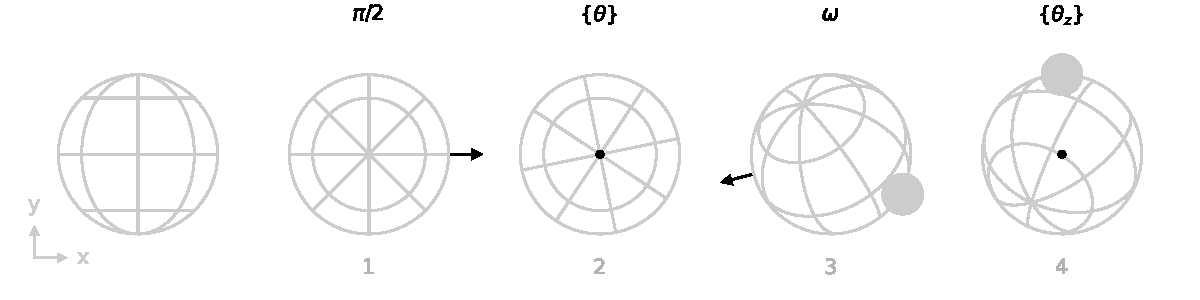
\includegraphics[width=\textwidth]{../workflows/rotations/figures/rotation_jaxoplanet_1.pdf}
        \caption{Consecutive rotations of the spherical harmonics basis in the \textsf{jaxoplanet} implementation. Each schematic shows a sphere rotated from a previous orientation around an axis displayed as a black vector and an angle shown on top.}
        \label{fig:rotation_jaxoplanet}
    \end{center}
\end{figure}

\subsection{Computation of the solution vectors}\label{solution_vectors}

In the general case, we described in \ref{model_occultation} how the integrated intensity of a spherical body occulted by another can be computed using the solution vector $\bvec{s}$. \cite{pal2012} shows that, knowing $\bvec{G}_n$, \autoref{eq:sn_gn} can be decomposed into
\begin{equation}
    s_n = \mathcal{Q}(\bvec{G}_n) - \mathcal{P}(\bvec{G}_n)
\end{equation}
where $\mathcal{Q}(\bvec{G}_n)$ and $\mathcal{P}(\bvec{G}_n)$ are line integrals over the contour of the occulting body parametrized by the angle $\varphi$ shown in \autoref{}\\\\


\begin{itemize}
    \item $\mathcal{Q}(\bvec{G}_n)$ is given by \citealt{starry} (Equation D28-29) in the general case, and is conveniently equal to $0$ for all $n > 0$ in the polynomial limb-darkening case.
    \item $\mathcal{P}(\bvec{G}_n)$ is given by \citealt{starry} (Equation D32), for the general case, and by \citealt{Agol2020} (Equation 71) in the polynomial limb-darkening case.
\end{itemize}
$\mathcal{P}$ and $\mathcal{Q}$ are given by \citealt[Equation D32]{starry}, for the general case, and \citealt[Equation 71]{Agol2020}, in the polynomial limb-darkening case


\begingroup\makeatletter\def\f@size{9}\check@mathfonts
$$
    \mbox{\normalsize$\mathcal{P}(\bvec{G}_n)$} =
    \begin{dcases}
        %
        2(2r)^{l+2}\int\displaylimits_{-\kappa/2}^{\kappa/2}
            (s_\varphi^2 -s_\varphi^4)^{\frac{\mu+4}{4}}
            (\delta + s_\varphi^2)^{\frac{\nu}{2}}
            \, \text{d}\varphi
            %
            & \qquad \frac{\mu}{2} \, \mathrm{even}
        \\[1em]
        %
        \mathcal{F}\int\displaylimits_{-\kappa/2}^{\kappa/2}
            (s_\varphi^2-s_\varphi^4)^{\tfrac{l-2}{2}}
            (k^2- s_\varphi^2)^{\frac{3}{2}}
            (1-2s_\varphi^2)
            \, \text{d}\varphi
            %
            & \qquad \mu = 1, \,
                     l \, \mathrm{even}
        \\[1em]
        %
        \mathcal{F}\int\displaylimits_{-\kappa/2}^{\kappa/2}
            (s_\varphi^2-s_\varphi^4)^{\tfrac{l-3}{2}}
            (\delta + s_\varphi^2)
            (k^2- s_\varphi^2)^{\frac{3}{2}}
            (1-2 s_\varphi^2)
            \, \text{d}\varphi
            %
            & \qquad \mu = 1, \, l \ne 1, \,
                     l \, \mathrm{odd}
        \\[1em]
        %
        2\mathcal{F}\int\displaylimits_{-\kappa/2}^{\kappa/2}
            (s_\varphi^2-s_\varphi^4)^{\frac{\mu-1}{4}}
            (\delta + s_\varphi^2)^{\frac{\nu-1}{2}}
            (k^2 - s_\varphi^2)^{\frac{3}{2}}
            \, \text{d}\varphi
            & \qquad \frac{\mu-1}{2} \, \mathrm{even}, \, l \ne 1
        \\[1em]
        %
        \int\displaylimits_{-\kappa/2}^{\kappa/2}
        r(r-b\cos{2\varphi})\;\frac{1-z^3}{3(1-z^2)}\text{d}\varphi & \qquad \mu=1, \, l=1
        \\[1em]
        %
        0 & \qquad \mathrm{otherwise},
    \end{dcases}
$$
\endgroup

\begingroup\makeatletter\def\f@size{9}\check@mathfonts
$$
    \mbox{\normalsize$s_n$} =
    \begin{dcases}
        %
        \pi - \kappa_1 - r^2\kappa_0 + \textit{A}_{kite} & \qquad n = 0
        \\[1em]
        \int\displaylimits_{-\kappa_0/2}^{\kappa_0/2}
        r(r-b\cos{2\varphi})\;\frac{1-z^3}{3(1-z^2)}\text{d}\varphi - \frac{2}{3}(\kappa_1 - \pi)& \qquad n = 1
        \\[1em]
        2s_0 + 4\pi\eta - 2\pi & \qquad n = 2
        \\[1em]
        2r(4br)^{\frac{n}{2}}
        \int\displaylimits_{-\kappa_0/2}^{\kappa_0/2}
        (k^2 - s_\varphi^2)^{\frac{n}{2}}
        (r - b + 2bs_\varphi^2) \, \text{d}\varphi & \qquad \mathrm{n\ge3},
    \end{dcases}
$$
\endgroup
    
\newpage
\section{Performance}\label{performances}
Although \textit{starry} occultation light curves have analytical expressions, their practical implementation relies on numerical approximations chosen to balance precision and computation time. This is the case, for example, of the solution vector $\bvec{s}$, computed using numerical series expansions in \textsf{starry} (\citealt[section D.2.3]{starry}) and numerical integration in \textsf{jaxoplanet} (see \autoref{solution_vectors}). Other expressions, such as the Wigner-D matrices used in the rotation of the spherical harmonics basis, are computed using reccurence relations prone to the accumulation of numerical errors and instability.\\\\
In this section, we evaluate the accuracy and speed of the \textsf{jaxoplanet} implementation and compare it with the C++ implementation of \textsf{starry}.

\subsection{Precision}
We evaluate the precision of the \textsf{starry} and \textsf{jaxoplanet} terms against quantities computed at arbitrary precision, using a ground truth version of the code implemented with the \texttt{mpmath} Python library\footlink{https://mpmath.org/}. The precision of the overall flux $f$ can only be understood by considering the precision of the terms involved in \autoref{eq:starry}: the solution vector $\bvec{s}$ ($\bvec{r}$ if no occultation), the basis matrices $\bvec{A}$ and $\bvec{B}$, and the Wigner-D rotation tensor $\bvec{R}$. Although we show in \autoref{fig:precision_SAR} that the precision of the \textsf{starry} and \textsf{jaxoplanet} implentations differ for many of these terms, we focus this section on the solution vector $\bvec{s}$ and the overall flux $f$.\\\\
Assuming that we perform the numerical integration of the solution vector $\bvec{s}$ at a relatively high order ($n=500$; see \autoref{solution_vectors}), \autoref{fig:precision_s} shows that our reimplentation of \textsf{starry} reaches relative errors lower than 1 part per billion for $\bvec{s}$ and the overall flux $f$, considering both a small ($r=0.01$) and a large ($r=100$) occultor transiting the star accross numerically-sensitive values of impact parameters $b$. For reference, \autoref{fig:precision_s_starry} shows comparable errors on the same quantities computed with the C++ implentation of \textsf{starry}. In addition, \autoref{fig:precision_degree} shows the evolution of the error on $f$ for increasing degrees of the spherical harmonics, both for \textsf{starry} and \textsf{jaxoplanet}. With these results, we validate the precision of \textsf{jaxoplanet} ans show it is on per with the legacy C++ \textsf{starry} implentation\footnote{version 1.2.0 \citep{starry_120}} described in \cite{starry}.\\\\
\begin{figure}[H]
    \begin{center}
        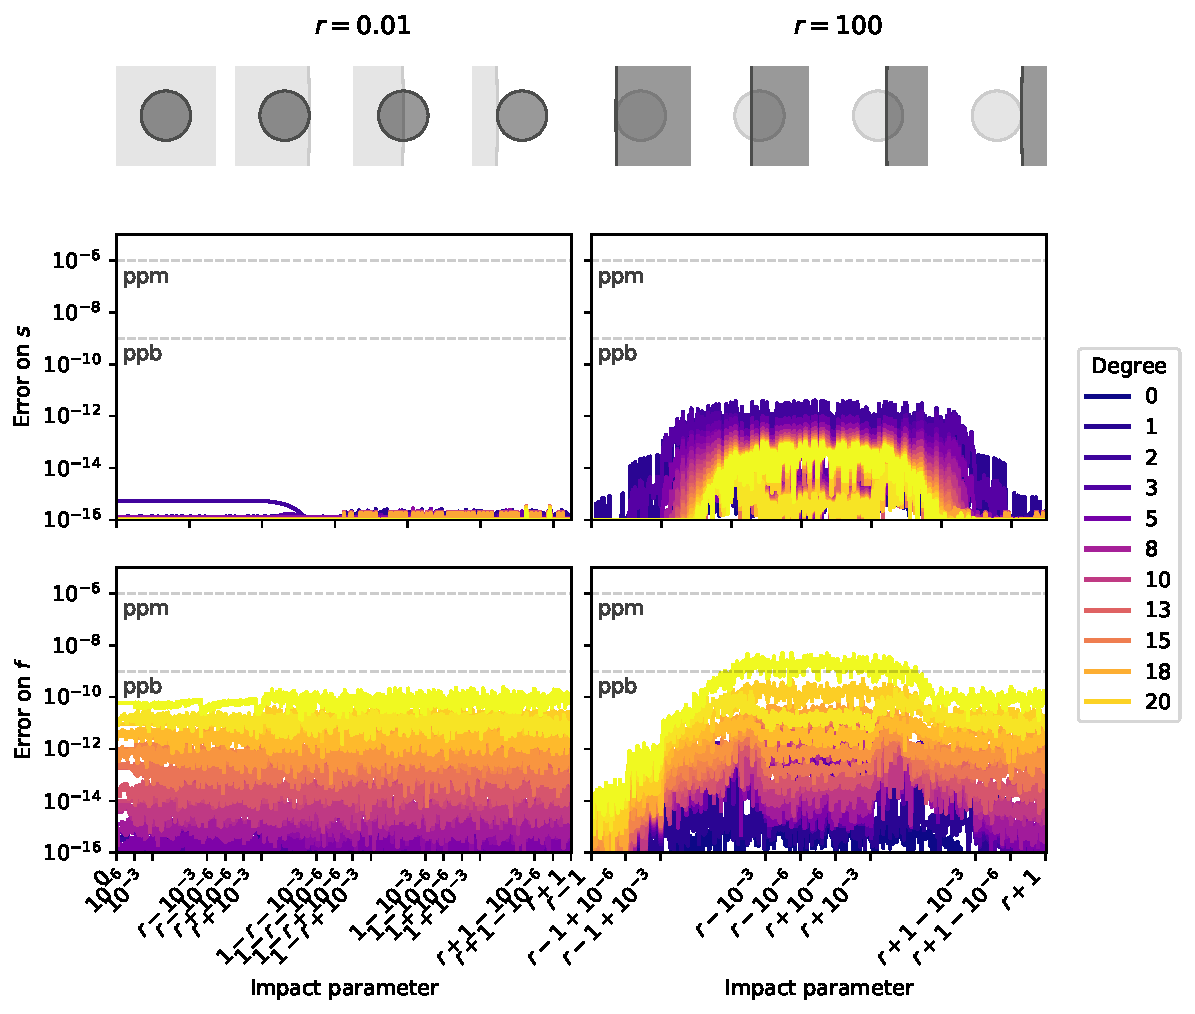
\includegraphics[width=\textwidth]{../workflows/precision/figures/error_jax.pdf}
        \caption{Error of the solution vector $\bvec{s}$ and the overall flux $f$ for all terms of the spherical harmonics basis up to degree $l=20$. Errors are computed against arbitrary-precision computations of $\bvec{s}$ and $f$ for a small ($r=0.01$) and a large ($r=100$) occultor transiting the star accross numerically-sensitive values of impact parameters $b$. For each $(l, m)$ basis component all coefficients are set to zero except $y_{l,m}=1$ and errors are scaled to the highest values of $\bvec{s}$ (respectively $f$) over $b$. Then, the plotted errors for each degree $l$ are the maximum of the scaled errors over all $m\in [-l, l]$ components over $b$. The disks at the top of the figure show the transit configurations of the occultor (light dark) and the star (light gray) for different values of $b$. \codelink{workflows/precision/scripts/plot_error}}
        \label{fig:precision_s}
    \end{center}
\end{figure}
\begin{figure}[H]
    \begin{center}
        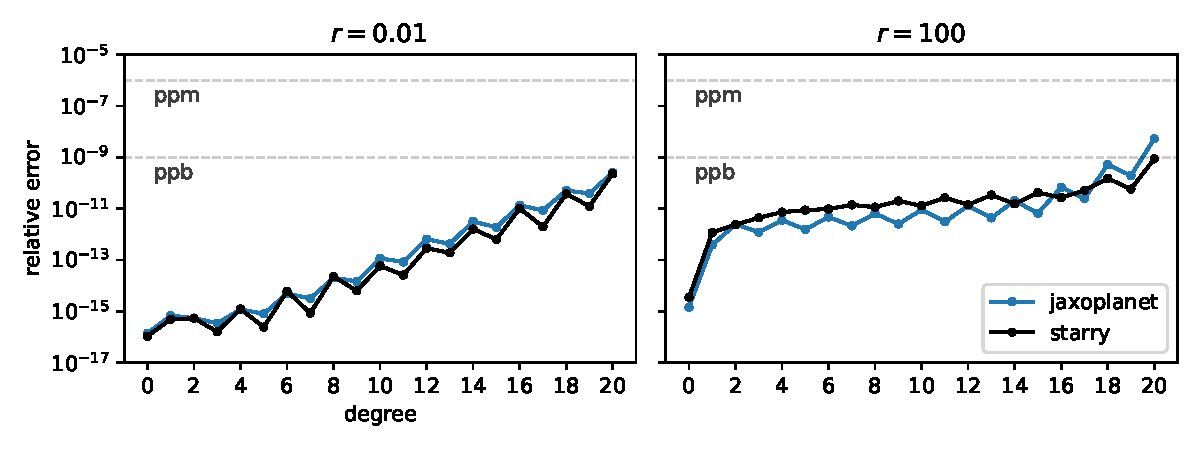
\includegraphics[width=\textwidth]{../workflows/precision/figures/error_degree.pdf}
        \caption{Maximum errors in the overall flux $f$ for all degrees of the spherical harmonics components. Errors shown in this figure correspond to the maximum values of the scaled errors shown in \autoref{fig:precision_s}, maxima taken over the range of values $b$. \codelink{workflows/precision/scripts/plot_error_vs_degree}}
        \label{fig:precision_degree}
    \end{center}
\end{figure}
For reference, \autoref{fig:precision_limbdark} shows the relative error in the flux of a limb-darkened star occulted by an opaque body for increasing orders of a polynomial limb-darkening law. In this figure, we also report the error of the flux computed using the \textsf{exoplanet} Python package (limited to linear and quadratic limb-darkening).
\begin{figure}[H]
    \begin{center}
        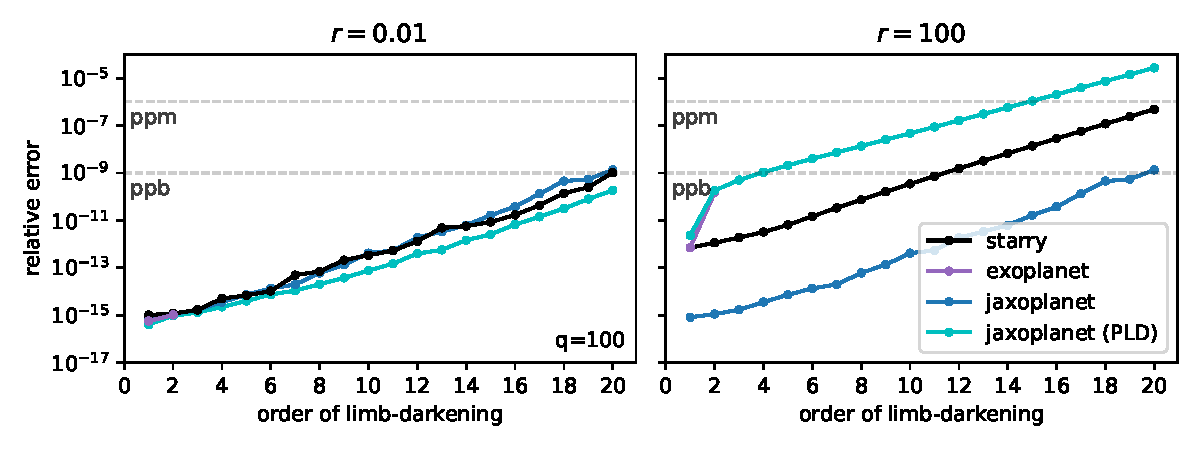
\includegraphics[width=\textwidth]{../workflows/precision/figures/limbdark_error.PDF}
        \caption{Maximum errors in the overall flux $f$ of a star occulted by an opaque body for increasing orders of its polynomial limb-darkening law. Errors shown in this figure correspond to the maximum values of the scaled errors shown in \autoref{fig:precision_s}, taken over the range of values $b$. For each order $n$ all limb-darkening coefficients are set to zero except the $n$-th coefficient $u_n=1$. \codelink{workflows/precision/scripts/plot_error_limbdark}}
        \label{fig:precision_limbdark}
    \end{center}
\end{figure}
A set of unitary polynomial limb-darkening coefficients of order 20 leads to spherical harmonics coefficients as large as $10^6$. This explains the larger errors observed in \autoref{fig:precision_limbdark} (error versus limb-darkening order) compared to the ones shown in \autoref{fig:precision_degree} (error versus degree of the spherical harmonics). We not that the errors scale with the values of $u$.\\\\
As described in \autoref{solution_vectors}, we compute \textit{starry} light curves using the Gauss Legendre quadrature to approximate the $\mathcal{P}$ integral involved in the expression of the solution vector $\bvec{s}$. Hence, the precision of the computed flux $f$ depends on the order of the Legendre polynomial which defines the number of points used to approximate $\mathcal{P}$. For this reason, users must carefully set the order parameter to reach the precision required for their application, as shown in \autoref{fig:relative_error_1}.\\\\
\begin{figure}[H]
    \begin{center}
        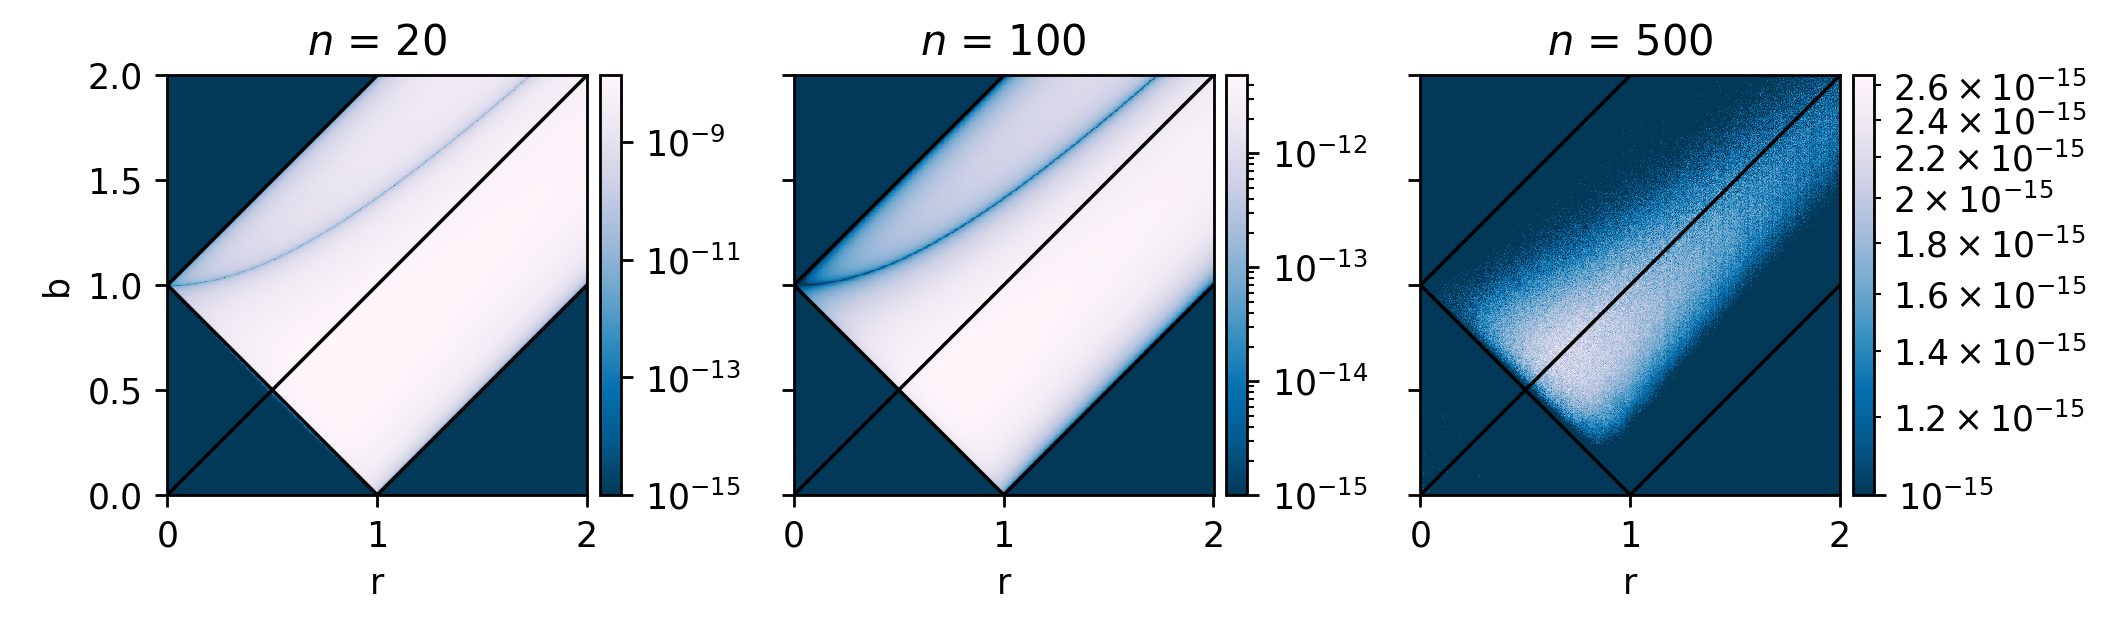
\includegraphics[width=\textwidth]{../workflows/precision/figures/br_error.png}
        \caption{relative numerical error in the flux $f$ of a linearly limb-darkened star (degree $l$=1) transited by an opaque companion over the $(r, b)$ parameter space. The error is evaluated for different orders $n$ of the Gauss-Legendre quadrature and computed against \textsf{starry} for speed and convenience. Note that \autoref{fig:precision_s} was produced using $n=500$ (right plot) for which $\bvec{s}$ reaches machine precision. \codelink{workflows/precision/scripts/plot_br_error}}
        \label{fig:relative_error_1}
    \end{center}
\end{figure}
In \autoref{fig:precision_order_gausslegendre}, we show how the error in the solution vector evolves with the order $n$ of the Gauss-Legendre quadrature, and its impact on the error in the overall flux.
\begin{figure}[H]
    \begin{center}
        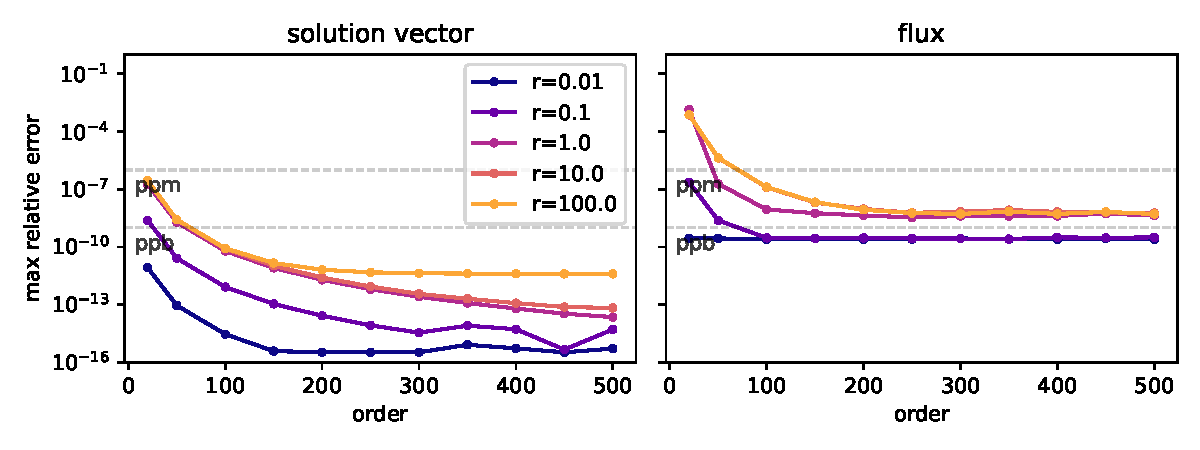
\includegraphics[width=\textwidth]{../workflows/precision/figures/error_order.pdf}
        \caption{Maximum errors in the solution vector and overall flux $f$ for different occultor radii and orders $n$ of the Gauss-Legendre quadrature used to compute the P integral (see \autoref{solution_vectors}). Errors shown in this figure correspond to the maximum values of the scaled errors shown in \autoref{fig:precision_s}, maxima taken over the range of values $b$. As in \autoref{fig:precision_s} the maximum degree of the spherical harmonics basis is set to $l=20$.}
        \label{fig:precision_order_gausslegendre}
    \end{center}
\end{figure}
The minimum error is always achieved for higher values of $n$, which comes with higher computational cost (see \autoref{speed}). Hence users must carefully set the order parameter to balance precision and computational speed. As the minimum error reached also depends on the degree of the spherical harmonics basis used, \autoref{fig:precision_order_gausslegendre_degree} shows the errors on the flux for each degree of the spherical harmonics basis, for an occultor with relative radii $r=0.01$, $r=1$ and $r=100$.
\begin{figure}[H]
    \begin{center}
        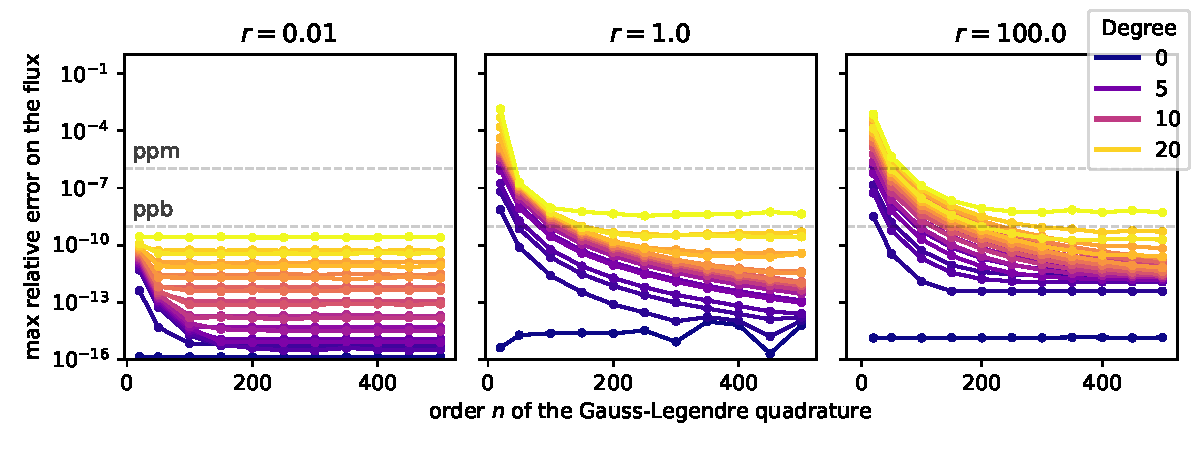
\includegraphics[width=\textwidth]{../workflows/precision/figures/error_order_degree.pdf}
        \caption{Maximum errors in the overall flux $f$ for all degrees of the spherical harmonics components for different occultor radii and orders $n$ of the Gauss-Legendre quadrature used to compute the P integral (see \autoref{solution_vectors}). Errors shown in this figure correspond to the maximum values of the scaled errors shown in \autoref{fig:precision_s}, maxima taken over the range of values $b$.}
        \label{fig:precision_order_gausslegendre_degree}
    \end{center}
\end{figure}
\subsection{Speed}\label{speed}

One of the advantage of the \texttt{JAX} library is its ability to perform hardware-accelerated computations on CPUs and GPUs. In this section, we evaluate the speed of the \textsf{jaxoplanet} implementation and compare it with the C++ implementation of \textsf{starry}. For quadratically limb-darkened light curve, we also compare our implementation with the one provided by the \textsf{exoplanet} Python package.\\\\
In \autoref{fig:speed_order_gausslegendre}, we show the evolution of the computing time required to compute an occultation light-curve of a limb-darkened star and that of a non-uniform star described by spherical harmonics with a maximum degrees $l=20$, depending on the order $n$ of the Gauss-Legendre quadrature used to compute the $\mathcal{P}$ integral numerically (see \autoref{solution_vectors}).\\\\
\begin{figure}[H]
    \begin{center}
        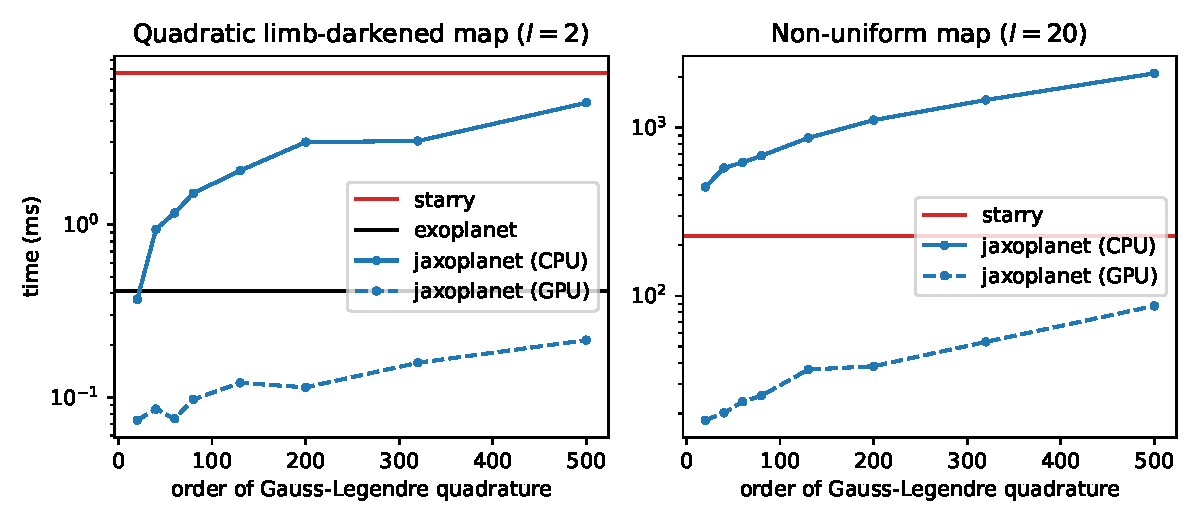
\includegraphics[width=\textwidth]{../workflows/speed/figures/speed_vs_order.pdf}
        \caption{Computation time of the occultation light curve of a limb-darkened star (left) and a non-uniform star described by spherical harmonics up to order $l=20$ (right) depending on the order $n$ of the Gauss-Legendre quadrature used to compute the P integral numerically (see \autoref{solution_vectors}). The processing time reported for \textsf{exoplanet} and \textsf{starry} is independent of $n$ as these two codes provide closed-form solutions for the integral $\mathcal{P}$. Light curves are computed for $10\,000$ points in transit and an occultor radius $r=0.1$.}
        \label{fig:speed_order_gausslegendre}
    \end{center}
\end{figure}
\begin{figure}[H]
    \begin{center}
        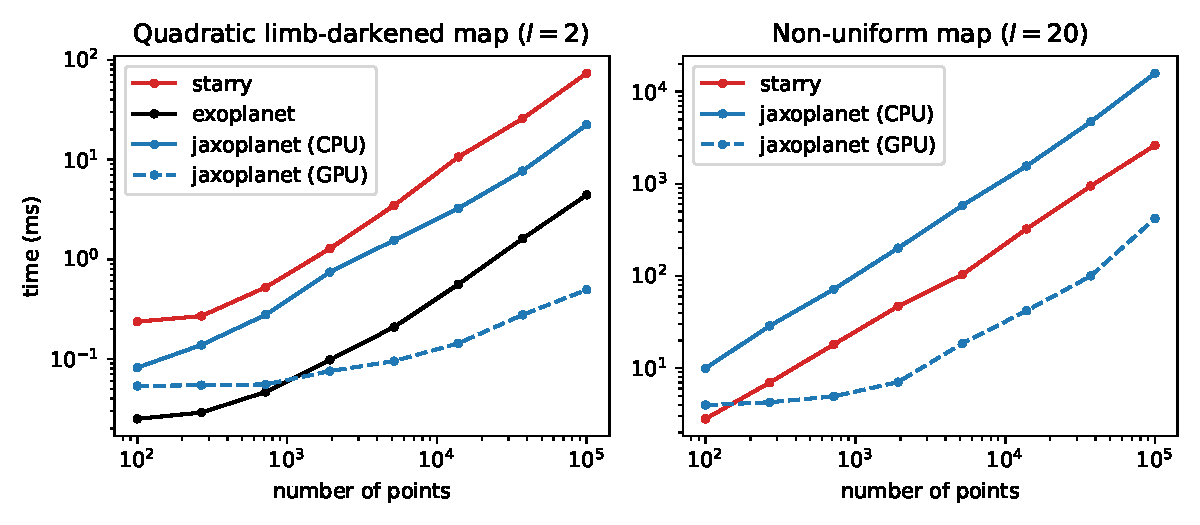
\includegraphics[width=\textwidth]{../workflows/speed/figures/speed_vs_N.pdf}
        \caption{Computation time of the occultation light curve of a limb-darkened star (left) and a non-uniform star described by spherical harmonics up to order $l=20$ (right) depending on the number of points in the light curve. Light curves are computed at order $n=200$ and an occultor radius $r=0.1$.}
        \label{fig:speed_N}
    \end{center}
\end{figure}
\autoref{fig:speed_order_gausslegendre}, in combination with \autoref{fig:precision_order_gausslegendre_degree}, can be used to determine a value of $n$ balancing precision and computation time.\\\\
Finally, \autoref{fig:speed_N} shows the evaluation time of \textsf{jaxoplanet} as a function of the number of points in the light curve, compared to \textsf{starry} for an $l=20$ surface map, and \textsf{exoplanet} for a quadratically limb-darkened star. As in the previous figure, we show that \textsf{jaxoplanet} is competitive against state-of-the-art codes on CPUs and offer a clear advantage on GPUs.



\section{Case studies: ...}

\subsection{}

\bibliography{ref}

\appendix

\section{Error budget}
\begin{figure}[H]
    \begin{center}
        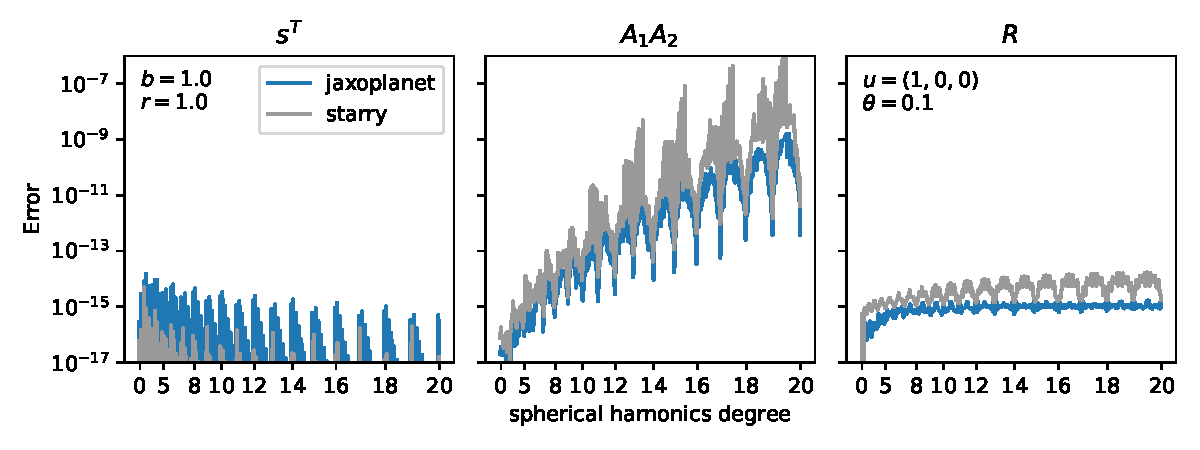
\includegraphics[width=\textwidth]{../workflows/precision/figures/error_SAR.pdf}
        \caption{\codelink{workflows/precision/scripts/plot_error_SAR}}
        \label{fig:precision_SAR}
    \end{center}
\end{figure}

\begin{figure}[H]
    \begin{center}
        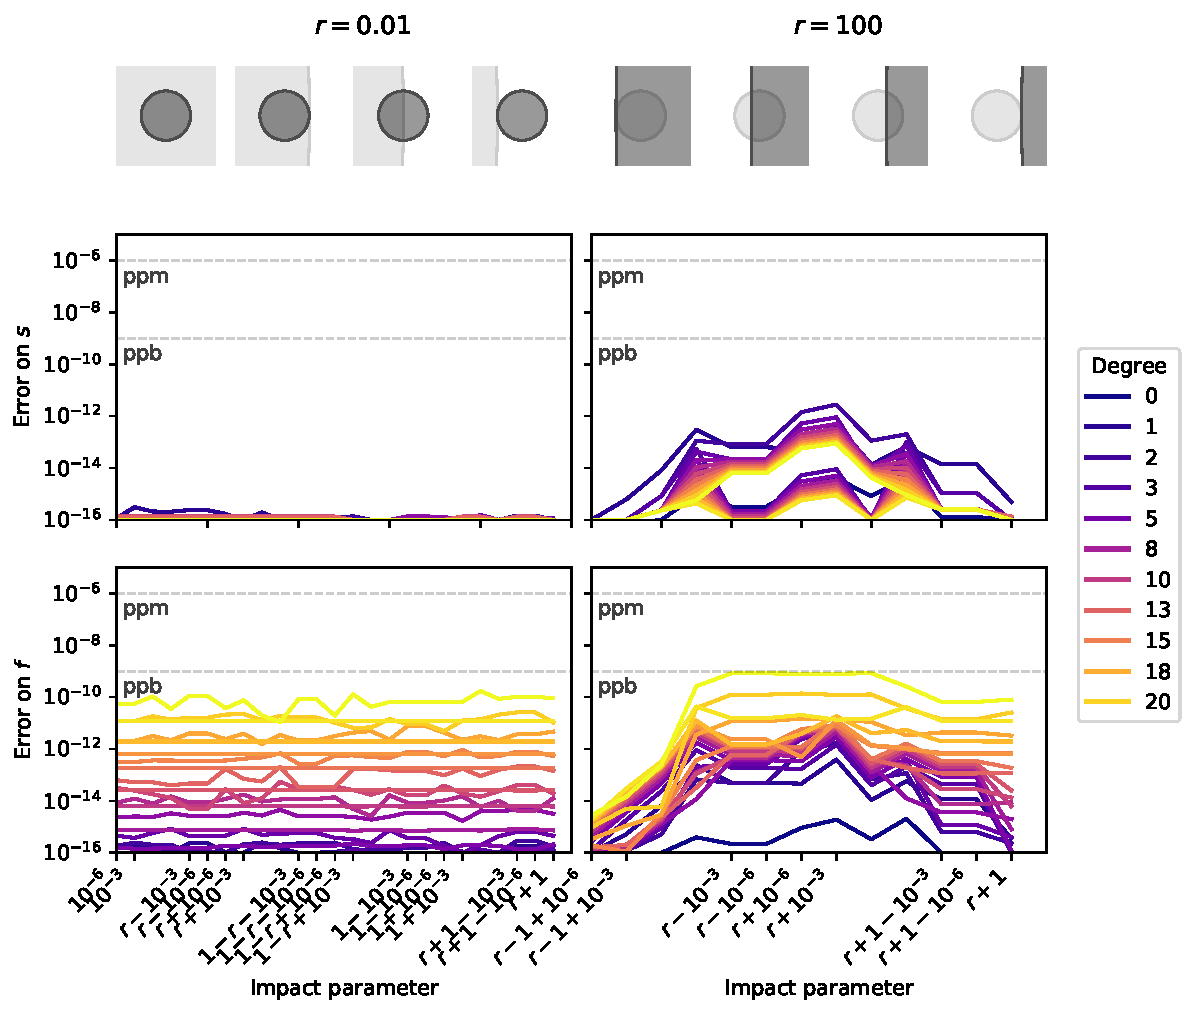
\includegraphics[width=\textwidth]{../workflows/precision/figures/error_starry.pdf}
        \caption{Same as \autoref{fig:precision_s} but with $bvec{s}$ and $f$ computed with the C++ implementation of \textsf{starry}. \codelink{workflows/precision/scripts/plot_error}}
        \label{fig:precision_s_starry}
    \end{center}
\end{figure}

% Table of symbols

\clearpage
\begin{center}
\renewcommand*{\arraystretch}{1.08}
\begin{longtable}{cll}
\caption{Symbols used in this paper} \label{tab:symbols} \\
%
\toprule
\multicolumn{1}{c}{\textbf{Symbol}} &
\multicolumn{1}{c}{\textbf{Definition}} &
\multicolumn{1}{c}{\textbf{Reference}} \\
\midrule
\endfirsthead
%
\multicolumn{3}{c}%
{{\bfseries \tablename\ \thetable{} --} continued from previous page} \\
\toprule
\multicolumn{1}{c}{\textbf{Symbol}} &
\multicolumn{1}{c}{\textbf{Definition}} &
\multicolumn{1}{c}{\textbf{Reference}} \\
\midrule
\endhead
\bottomrule
%
\endfoot
%
\bottomrule
\endlastfoot
%
$\omega$        & Rotation angle of the combined rotation       & \autoref{eq:combined_angle} \\
$n$ & order of the Gauss-Legendre approximation & \\
$r$ & occultor radius in units of occulted body's radius & \\
%
\end{longtable}
\end{center}

\end{document}